\documentclass[11pt,a4paper]{article}
\usepackage[utf8]{inputenc}
\usepackage{amsmath}
\usepackage{amsfonts}
\usepackage{amssymb}
\usepackage[left=1cm,right=1cm,top=2cm,bottom=2cm]{geometry}
\usepackage{graphicx}
\usepackage{hyperref}

\author{Théo Gouzien - Théo Losekoot}
\title{Rapport de projet DSL}

\begin{document}

\maketitle

\section{Introduction et méthode}

Dans ce rapport, nous allons rapporter les performances de différentes versions des solveurs \textit{SAT4J}, \textit{MiniSAT} et \textit{CryptoMiniSAT}.
Pour ce faire, nous utiliserons la base de donnée de formules booléennes trouvable à cet url : \url{https://github.com/diverse-project/samplingfm/tree/master/Benchmarks}.
Plus précisément, nous utiliserons uniquement les 70 fichiers .cnf qui sont dans le répertoire "Benchmarks" de cette base de données.

Les solveurs testés sont : 
\begin{itemize}
\item SAT4J - version 2.3.1 - JAR exécutable - paramètres par défaut 
\item -----------------------------------
\item MiniSAT - version 1.14.0 - binaire - paramètres par défaut
\item MiniSAT - version 2.2.0  - binaire - -rnd-freq=0 (Défaut)
\item MiniSAT - version 2.2.0  - binaire - -rnd-freq=0.5
\item MiniSAT - version 2.2.0  - binaire - -rnd-freq=0.9
\item -----------------------------------
\item CryptoMiniSAT - version 2.4.0 - binaire - paramètres par défaut
\item CryptoMiniSAT - version 3.1.0 - binaire - paramètres par défaut
\item CryptoMiniSAT - version 4.5.3 - binaire - paramètres par défaut
\item CryptoMiniSAT - version 5.6.8 - binaire - --freq=0 (Défaut)
\item CryptoMiniSAT - version 5.6.8 - binaire - --freq=0.5
\item CryptoMiniSAT - version 5.6.8 - binaire - --freq=0.9
\end{itemize}

Afin de comparer ces solveurs, nous récupérons leur résultat et leur temps d'exécution sur toutes les formules du dossier "Benchmarks", avec un timeout à 10 minutes. 
Afin d'obtenir des résultats les moins bruités possible, nous effectuons ces calculs plusieurs fois et utilisons la moyenne.

Les tests sont lancés depuis un projet XText. Pour reproduire les données présentées dans ce rapport, il suffit d'exécuter le fichier "org.xtext.example.msat.tests/src/org/xtext/example/msat/theos/Mein.xtend" avec JUnit. Les résultats seront stockés dans les fichiers "result\_\textit{i}.csv".

Au total, les benchmarks ont duré 20 heures, avec six itérations par test.


\section{Résultats}

Les données brutes peuvent être trouvées dans le dossier "results", avec "results\_\textit{i}.csv" les données de chaque exécution de la base de données.
Toutes les données discutées ensuite sont extraites et ré-extractibles des fichiers "results\_\textit{i}.csv" grâce au script python "get\_infos.py". 
Les mesures de temps ont été récupérées dans la sortie standard des solveurs, afin de minimiser l'importance des conditions d'exécution. Les temps sont directement inscrits dans les fichiers csv correspondants.

\subsection{Aspect fonctionnel}

Tous les solveurs ayant eu le temps de terminer dans leur temps imparti ont renvoyé la même réponse pour toutes les formules présentes dans "Benchmarks".

À noter que dans les cas où les solveurs ont timeout il se pourrait qu'il existe en réalité un bug mais que les conditions de tests ne nous aient pas permis de le découvrir. Par exemple, pour la formule \textit{listReverse.sk\_11\_43}, le solveur Sat4J a timeout systématiquement.

\subsection{Efficacité}

Afin de comparer l'efficacité, nous ne parlerons ici que du temps d'exécution, sans tenir compte d'autres facteurs tels que l'espace utilisé. Afin de faciliter les calculs, nous considérons que un solveur ayant échoué pour cause de timeout correspond à un calcul de 15 minutes. Cela ne s'éloigne pas beaucoup de la réalité sur les formules traitées ici et a un faible impact pour cause du faible nombre de timeout.

La table \ref{tab:results} récapitule les résultats que nous avons trouvé pertinent de mettre en avant. 
La colonne "Premier" indique combien de fois le solveur a fini avant les autres. Le total ne s'additionne pas à 70 car nous n'avons pas pris en compte les formules que tous les solveurs traitaient en moins de 0.01s, car le temps est trop court pour être pertinent.
La colonne "Timeout" indique le nombre de timeout effectué par chacun de ces solveurs, sur les $70 * 6$ formules traitées. 

\begin{table}[]
\begin{tabular}{|l|l|l|l|l|l|}
\hline
Solveur       & Version & Paramètres    & Premier & Temps moyen        & Timeout \\ \hline
SAT4J-Jar     & 2.3.1   &               & 0       & 35.713  & 8       \\
MiniSAT       & 1.14.0  &               & 0       & 30.909  & 8       \\
MiniSAT       & 2.2.0   & -rdn-freq=0   & 5       & 28.380 & 8       \\
MiniSAT       & 2.2.0   & -rdn-freq=0.5 & 8       & 21.301 & 4       \\
MiniSAT       & 2.2.0   & -rdn-freq=0.9 & 1       & 28.466 & 8       \\
CryptoMiniSAT & 2.4.0   &               & 0       & 24.241 & 5       \\
CryptoMiniSAT & 4.5.3   &               & 3       & 4.498  & 0       \\
CryptoMiniSAT & 5.6.8   & --freq=0      & 3       & 10.498 & 0       \\
CryptoMiniSAT & 5.6.8   & --freq=0.5    & 1       & 20.116 & 4       \\
CryptoMiniSAT & 5.6.8   & --freq=0.9    & 1       & 20.639 & 4       \\ \hline
\end{tabular}
\caption{Resultats sur les 70 formules de "Benchmarks"}
\label{tab:results}
\end{table}


\section{Questions}

\subsection{Le ``meilleur" solveur ?}

Le temps moyen de résolution pour toutes les formules est trouvable dans la table \ref{tab:results}.


On remarque que MiniSAT termine souvent premier, voir fig \ref{fig:first}, mais que CryptoMiniSAT 4.5.3 a un bien meilleur temps moyen, voir fig \ref{fig:mean}. Cela s'explique par le fait que CryptoMiniSAT a un bien meilleur temps sur les instances difficiles, mais se fait en moyenne battre sur les faibles instances.
Lorsque CryptoMiniSAT 4.5.3 finit en premier, alors il a en moyenne 74.7 secondes d'avance, et lorsqu'il ne finit pas en premier, il a en moyenne seulement 2.3 secondes de retard.
On note que SAT4J-Jar n'est ni en tête au niveau du temps moyen, ni en tête au niveau d'exécutions les plus rapides, mais a le bon goût de posséder une API Java ainsi qu'un JAR facilement exécutable.

Il n'y a donc pas de meilleur solveur en tout point, mais seulement des solveurs plus adaptés à certaines situations. À noter tout de même que CryptoMiniSAT est très proche de MiniSAT sur des instances faciles, et est donc presque strictement mieux que ce dernier.

Nos propos sont tout de même à nuancer.
En effet, les SAT-solveurs modernes utilisent des heuristiques qui peuvent légèrement varier et, pour des instances particulières, mener à des écarts de performances plus ou moins importants. De fait, la question du "meilleur" solveur n'a pas tant de sens sans ces guillemets. Cependant dans notre cas, au vu des informations à notre disposition, la réponse n'appelle pas particulièrement à la nuance :

Sur cet ensemble de tests, CryptoMiniSAT 4 domine largement le reste des solveurs.
Il est d'ailleurs étonnnt de constater que la version 4 a de bien meilleurs résultats que la version 5. Une explication possible est que la version 5 a été optimisée pour de très grandes instances et que notre timeout de 10 minutes (ainsi que notre ensembles de tests limité) ne permet pas de mettre en valeur ces cas de figures. Des tests plus répétés, plus variés, et plus longs seraient donc nécessaires pour justement évaluer ces solveurs.

\begin{figure}
  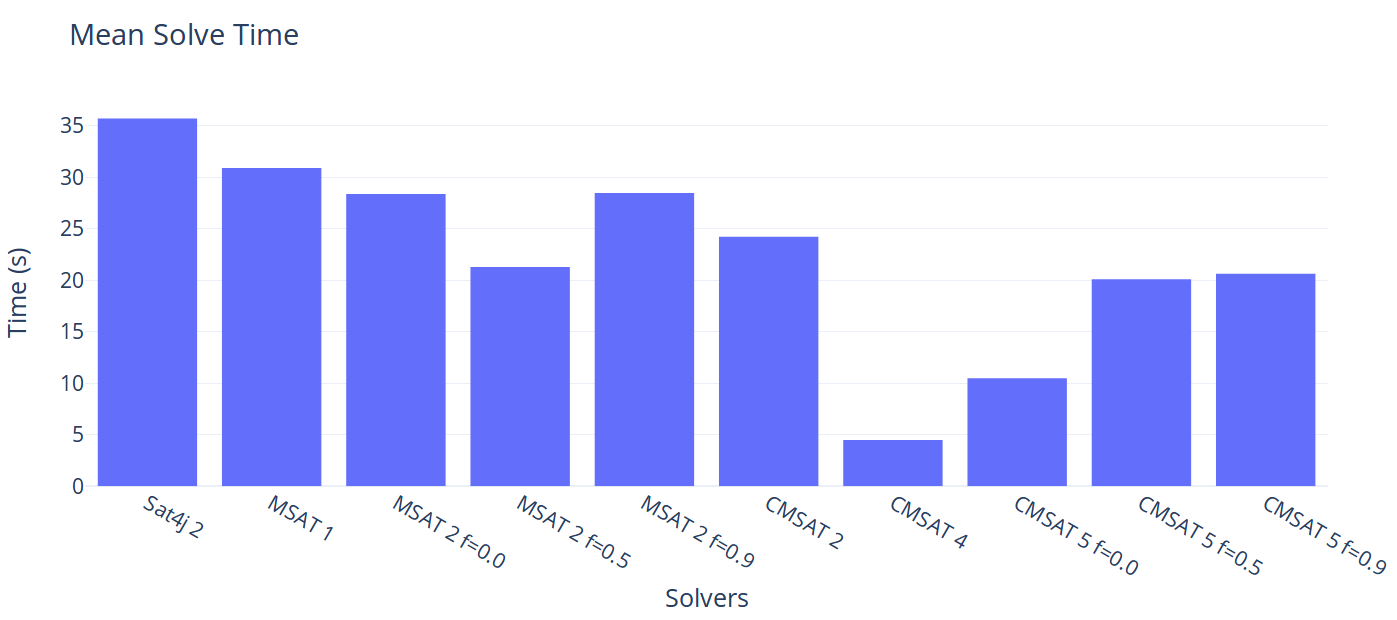
\includegraphics[width=0.6\linewidth]{plot-mean.png}
  \caption{Temps moyen, sur les 6 répétitions, de l'exécution des solveurs sur l'ensemble des 70 formules. }
  \label{fig:mean}
\end{figure}

\begin{figure}
  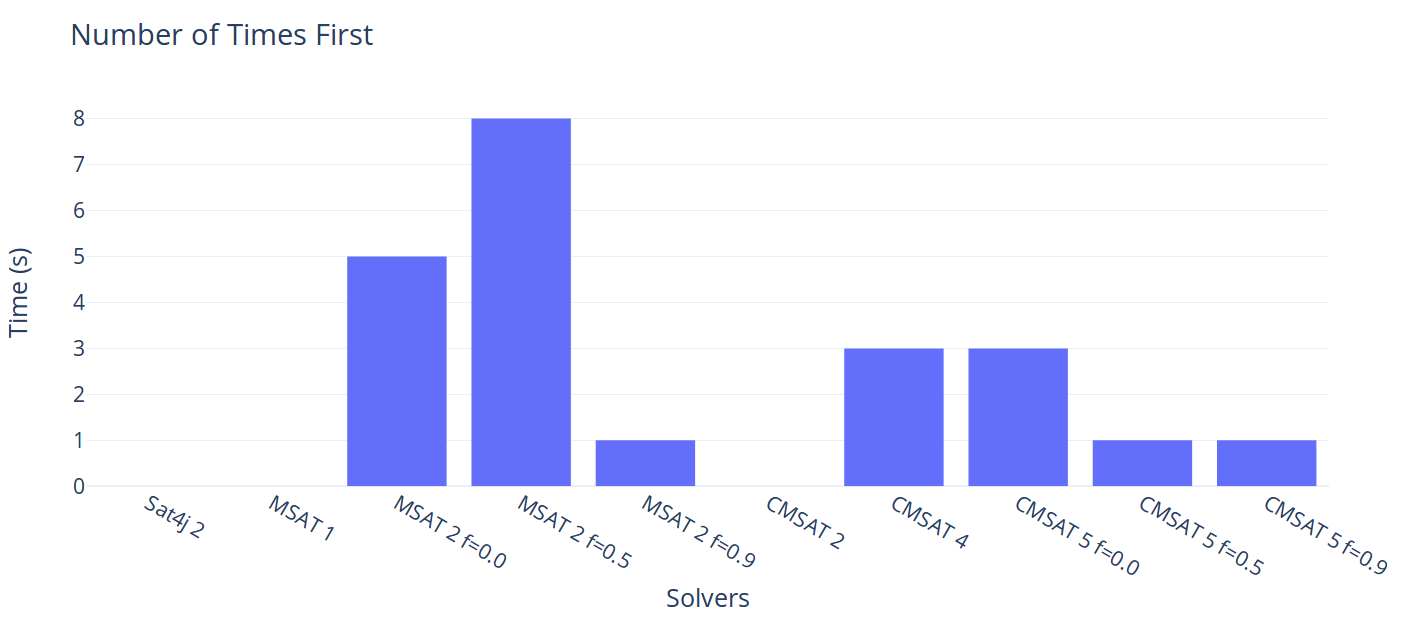
\includegraphics[width=0.6\linewidth]{plot-first.png}
  \caption{Nombre de fois qu'un solveur s'arrête avant les autres, sur le temps moyen des solveurs sur les 70 formules.}
  \label{fig:first}
\end{figure}

\subsection{L'existence de bugs}
 
Outre les bugs visibles par les sorties fonctionnelles, nous pourrions essayer de repérer un bug par un temps d'exécution anomal. On peut considérer un temps d'exécution d'un certain solveur sur une certaine formule comme anormal s'il dévie trop d'une exécution à l'autre. Nous n'avons pas trouvé ce genre de déviations dans nos données. 
La comparaison de temps entre solveurs n'est pas une très bonne mesure de détection de bugs. En effet, certains solveurs sont juste moins efficaces sur certaines instances sans pour autant que ce soit un bug.


\subsection{La difficulté des formules}

 La signification de "formule plus difficile" peut être comprise de plusieurs manières. On pourrait penser à une formule qui prend plus de temps à être résolue, peu importe la méthode employée, ou encore à une formule simple une fois que la bonne méthode est trouvée (ce qui est difficile). 
 Il n'existe pas de formule universellement plus difficile que les autres. On peut néanmoins exhiber certains signes de difficulté ou de facilité des formules. 
 Une formule très courte est nécessairement simple. Même le brute-force est rapide.
 Une formule longue peut être simple ou plus difficile. Par exemple, si elle contient une contradiction immédiate, comme une clause "1 0" ainsi qu'une autre clause "-1 0", alors peu importe sa longueur, sa solution est assez rapide à calculer. Dans les SAT solveurs modernes, des techniques sophistiquées sont employées pour ne pas avoirà brute-force. Ces techniques, et je pense principalement ici au "clause-learning", exploitent la structure du problème. En effet, une instance décrivant un système réel sera très probablement plus simple qu'une instance aléatoire de même taille. 
De plus, les solveurs peuvent être spécialisés dans certains types d'instances (SAT/UNSAT, ALÉATOIRE/RÉEL, etc...).
La difficulté des formules n'est donc pas un ordre total, mais il est courant d'avoir des instances prenant plus de temps sur l'ensemble des solveurs connus que d'autres instances. Par exemple, dans notre base de données "Benchmarks", la formule \textit{listReverse.sk\_11\_43} est la plus longue à calculer.



\subsection{De meilleures benchmarks ?}

En fonction du type de solveur que l'on est train de tester ainsi que de la particularité (fonctionnel, efficacité temporelle, efficacité mémoire, etc.), il est sûrement possible de se ramener à un sous-ensemble de formules. Néanmoins, des formules ayant une faible variation de performance peuvent tout de même être utiles, soit pour la comparaison aux autres solveurs, soit pour avoir des repères lors de l'intégration continue de prochaines heuristiques. 
Dans notre cas, une grande diversité dans la base de donnée est requise car nous souhaitons vraiment observer les points forts de chaque solveur.


\end{document}